\documentclass[journal]{IEEEtran}

\usepackage{amsmath}
\usepackage{array}
\usepackage{cite}
\usepackage{graphicx}
\usepackage{url}

\ifCLASSINFOpdf
  \graphicspath{{figures/}}
  \DeclareGraphicsExtensions{.pdf,.png,.jpg,.jpeg}
\else
  \graphicspath{{figures/}}
  \DeclareGraphicsExtensions{.eps}
\fi

\hyphenation{Web-Assembly Gray-Scott auto-dif-fer-en-ti-a-tion}

\begin{document}

\title{Differentiable Gray--Scott Reaction--Diffusion in WebAssembly}

\author{Rohit~Kumar%
\thanks{R. Kumar is with Lovely Professional University. E-mail:
rohitkumar.20246@lpu.in.}}

\markboth{Kumar: Differentiable Gray--Scott in WebAssembly}%
{Kumar: Differentiable Gray--Scott in WebAssembly}

\maketitle

\begin{abstract}
Reaction--diffusion systems are compact nonlinear benchmarks for browser
simulation, visualization, and inverse parameter recovery. This paper presents a
Rust and WebAssembly implementation of the Gray--Scott model with deterministic
validation against Python and NumPy references, render-path measurements,
WebAssembly SIMD acceleration, and differentiable inverse recovery for the feed
and kill parameters. On the two-parameter inverse task, forward-mode gradients
cost about \(2.6\times\) a primal loss evaluation on production-relevant native
grids, compared with about \(5.0\times\) for central finite differences. The
WASM SIMD build achieves \(7.0\times\)--\(8.6\times\) speedup over scalar WASM
in Node.js. The backtracking AD optimizer reaches lower clean field loss than a
dense grid search while using 17 evaluations rather than 1581 candidates, and
it completes a \(64\times64\) inverse recovery in 68 ms in-browser via a Web
Worker, without GPU, Python, or server-side compute. Noise sweeps show stable
grid recovery through uniform noise amplitude 0.020 and degradation by
0.050--0.100. These results support WebAssembly as a practical target for
interactive differentiable reaction--diffusion experiments while clarifying the
limits of two-parameter forward-mode AD and single-browser performance
measurements.
\end{abstract}

\begin{IEEEkeywords}
Reaction--diffusion, Gray--Scott model, WebAssembly, automatic
differentiation, inverse problems, scientific visualization.
\end{IEEEkeywords}

\IEEEpeerreviewmaketitle

\section{Introduction}
\IEEEPARstart{R}{eaction--diffusion} systems provide a useful middle ground
between toy numerical kernels and full scientific simulation codes. They are
small enough to run interactively in a browser, but their nonlinear dynamics
make validation, visualization, and inverse recovery nontrivial. The Gray--Scott
model~\cite{gray1984autocatalytic} is especially attractive because simple
changes in the feed parameter \(F\) and kill parameter \(k\) produce visibly
different pattern regimes.

This work asks whether a browser-deliverable implementation can support more
than visualization: can it also expose enough numerical structure for credible
inverse experiments? The implementation targets Rust for native validation and
WebAssembly deployment~\cite{webassemblycore2}. The inverse task is to recover
\(F\) and \(k\) from a final simulated pattern under a fixed initial condition.

The contributions are:
\begin{itemize}
  \item a deterministic Rust/WebAssembly Gray--Scott solver validated against
  scalar Python and NumPy \texttt{float32} references;
  \item a browser render benchmark separating field-to-RGBA conversion,
  \texttt{ImageData}, \texttt{putImageData}, and OffscreenCanvas costs;
  \item a forward-mode AD implementation for two-parameter inverse recovery;
  \item an empirical comparison of dense grid search, finite differences, fixed
  step AD, and Armijo backtracking AD under deterministic target noise;
  \item a WASM \texttt{simd128} forward kernel achieving
  \(7.0\times\)--\(8.6\times\) speedup over scalar WASM across
  \(128^2\)--\(512^2\) grids in Node.js;
  \item a browser inverse page executing the full AD optimizer off the main
  thread via a Web Worker.
\end{itemize}

\section{Background}
\subsection{Reaction--Diffusion Pattern Formation}
Reaction--diffusion pattern formation is usually traced to Turing's chemical
basis of morphogenesis~\cite{turing1952morphogenesis}, which showed how
diffusion and local reaction kinetics can destabilize a homogeneous state.
Pearson later demonstrated that the Gray--Scott system produces a wide range of
complex spatiotemporal patterns despite its compact two-species form
~\cite{pearson1993complex}. Broader reaction--diffusion theory connects these
systems to biological pattern formation, nonlinear chemical dynamics, and
parameter-space structure~\cite{murray1982parameter,murray2003mathematical,
koch1994biological,epstein1998nonlinear}. This makes Gray--Scott a useful
benchmark: it has simple equations, but its final patterns are nonlinear enough
to make inverse parameter recovery nontrivial.

\subsection{Gray--Scott Model}
The Gray--Scott system describes two reacting and diffusing chemical species,
commonly written as
\begin{align}
  \frac{\partial u}{\partial t} &= D_u \nabla^2 u - uv^2 + F(1-u), \\
  \frac{\partial v}{\partial t} &= D_v \nabla^2 v + uv^2 - (F+k)v.
\end{align}
Here \(u\) and \(v\) are concentration fields, \(D_u\) and \(D_v\) are diffusion
coefficients, \(F\) is the feed rate, and \(k\) is the kill rate. This paper uses
an explicit finite-difference update with periodic boundaries and a deterministic
square seed.

\begin{figure}[!t]
\centering

\includegraphics[width=2.6in]{gray_scott_pattern}
\caption{Developed \(v\)-field pattern generated with \(F=0.060\),
\(k=0.062\), a \(256\times256\) grid, and 1000 steps. This visualization is
separate from the smaller inverse-recovery benchmark and is included to show a
recognizable Gray--Scott pattern regime.}
\label{fig:pattern}
\end{figure}

\subsection{Inverse Recovery}
Given a target final field \((u^\star, v^\star)\), the inverse objective is mean
squared error over both fields:
\begin{equation}
  L(F,k) =
  \frac{1}{2N}\sum_{i=1}^{N}\left[
    (u_i(F,k)-u_i^\star)^2 + (v_i(F,k)-v_i^\star)^2
  \right].
\end{equation}
The experiments compare dense grid search, central finite differences, and
forward-mode AD for minimizing this objective.

\subsection{WebAssembly for Scientific Kernels}
WebAssembly was designed as a compact, safe, low-level compilation target for
the Web with predictable validation and execution semantics
~\cite{haas2017webassembly,webassemblycore2}. Prior work positions it as a
portable target for performance-sensitive browser applications rather than a
replacement for native HPC. This paper uses that positioning directly: Rust is
used for reproducible native tests, while the same solver is exported to
WebAssembly for browser deployment and rendering measurements.

\subsection{Differentiable PDE and Physics Frameworks}
Differentiable physics systems such as DiffTaichi~\cite{hu2020difftaichi},
JAX and JAX~MD~\cite{bradbury2018jax,schoenholz2021jaxmd}, JAX-Fluids
~\cite{bezgin2023jaxfluids,bezgin2025jaxfluids2}, and
\(\Phi_{\mathrm{Flow}}\)~\cite{holl2024phiflow} show that automatic
differentiation can be integrated into simulation codes for optimization,
learning, and inverse problems. Other work uses differentiable PDE solvers as
training components for control and learning~\cite{holl2020controlpdes,
um2020solverloop,raissi2019pinns}. This paper is narrower: it does not attempt a
general differentiable PDE framework, but instead measures a small
forward-mode AD path for a browser-deliverable Gray--Scott solver.

\subsection{Browser PDE Tools}
Interactive browser PDE tools already show the value of immediate simulation and
visual exploration. VisualPDE provides rapid browser-based PDE simulations for
education and exploration~\cite{walker2023visualpde}. The contribution here is
complementary: instead of emphasizing general interactive modeling, the system
couples a WebAssembly Gray--Scott implementation with native validation,
render-path measurements, and a small differentiable inverse-recovery benchmark.

\section{Implementation}
\subsection{Solver}
The solver is implemented in Rust with \texttt{f32} fields. The same core update
is used for native validation and WebAssembly exports. The browser interface
exposes copied fields and zero-copy \texttt{Float32Array} views into WASM memory.
The primal solver stores the two concentration fields in separate contiguous
arrays, \(u\) and \(v\), with matching scratch arrays for the next time step.
This structure-of-arrays layout keeps the five-point Laplacian stencil simple:
each update reads the center, left, right, up, and down entries from one field
at a time, writes the corresponding next-field entry, and swaps buffers after a
complete step. Periodic boundaries are handled by index wrapping at the stencil
accesses, so the storage layout is identical for native and WebAssembly builds.

The WebAssembly interface exposes two kinds of field access. The copied accessors
return owned JavaScript arrays and are useful for API safety and testing. The
zero-copy accessors return \texttt{Float32Array} views over the module memory,
avoiding a full field copy across the JavaScript--WebAssembly boundary. Because
views into WebAssembly memory can be invalidated if memory grows, rendering code
recreates the views after operations that may allocate. The benchmarked browser
rendering path uses the zero-copy field view as input, converts the selected
field to a reusable RGBA buffer, then measures \texttt{ImageData} construction
and canvas upload separately.

The differentiated solver uses the same grid traversal and boundary handling,
but each scalar value carries a primal component and two tangent components. The
current implementation keeps this dual representation as a direct, readable
extension of the scalar solver rather than introducing a separate optimized
tangent-memory layout. This choice favors validation and paper reproducibility;
the measured overhead in Section~V shows where memory traffic begins to matter.

A separate \texttt{simd128} build provides a SIMD-accelerated forward kernel.
Interior rows use 4-wide \texttt{f32x4} operations; boundary rows use the scalar
path to preserve periodic-boundary correctness. The two builds share the same
field layout and are validated against each other before benchmarking.
Scalar-vs-SIMD maximum field delta is below \(8\times10^{-7}\); the small
checksum difference of \(3.2\times10^{-9}\) relative error results from SIMD
lane operation reordering.

The browser inverse page executes the AD optimizer inside a module Web Worker
via \texttt{www/inverse\_worker.js}, keeping the main browser thread free during
recovery. The worker initializes the WASM module independently and returns a
JSON result including optimizer history and a \texttt{worker: true} flag
confirming off-thread execution.

All code, benchmark scripts, and raw results are available at
\url{https://github.com/itisrohit/grayscott-wasm}.

\subsection{Forward-Mode AD}
For the inverse task, each scalar value carries a primal value and two tangent
components, one for \(F\) and one for \(k\), following standard forward-mode
automatic differentiation~\cite{rall1981automatic,griewank2008evaluating,
bartholomew2000automatic,pearlmutter1994fast,baydin2018automatic}. This directly
computes \(\partial L/\partial F\) and \(\partial L/\partial k\) in one
differentiated simulation. For two parameters this is expected to be cheaper than
central finite differences, which require five primal evaluations per gradient
query.

\subsection{Backtracking Optimizer}
The AD optimizer uses steepest descent with Armijo backtracking line
search~\cite{armijo1966minimization,nocedal2006numerical}. A candidate step
starts from \(\alpha_0 = 10^{-3}\), shrinks by \(0.5\), and is
accepted when
\begin{equation}
  L(x+\alpha p) \le L(x) + c\alpha \nabla L(x)^T p,
\end{equation}
with \(c=10^{-4}\) and \(p=-\nabla L(x)\). This adds a small number of primal
loss evaluations but avoids the brittle learning-rate behavior observed with a
fixed step.

\section{Experimental Setup}
All inverse experiments use a \(64\times64\) grid, 100 simulation steps, a
deterministic centered square seed, \(D_u=0.16\), \(D_v=0.08\), and \(dt=1\).
The default off-grid target is \(F=0.06055\), \(k=0.06245\). Dense grid search
uses \(F\in[0.045,0.070]\) with 51 samples and \(k\in[0.055,0.070]\) with 31
samples, for 1581 candidates.

Noise sensitivity is tested by adding deterministic independent uniform noise
to both target fields and clamping values to \([0,1]\). Four seeds are used at
noise amplitudes 0.000, 0.020, 0.050, and 0.100 for the AD optimizer comparison.

\section{Results}
\subsection{Correctness Validation}
Full-field comparisons against NumPy \texttt{float32} references show small
absolute error across tested regimes. Table~\ref{tab:correctness} reports the
four \(64\times64\) regimes tested at 1000 steps. The largest observed maximum
error is below \(4\times10^{-5}\), occurring in the more sensitive
\(F=0.050\), \(k=0.065\) regime.

\begin{table*}[!t]
\renewcommand{\arraystretch}{1.15}
\caption{Full-Field Rust vs. NumPy \texttt{float32} Validation at 1000 Steps}
\label{tab:correctness}
\centering
\begin{tabular}{lcccccc}
\hline
Regime & \(u\) MAE & \(v\) MAE & \(u\) RMSE & \(v\) RMSE & \(u\) MaxErr & \(v\) MaxErr\\
\hline
\(F=0.037, k=0.060\) & \(1.697{\times}10^{-7}\) & \(1.002{\times}10^{-7}\) & \(2.714{\times}10^{-7}\) & \(1.794{\times}10^{-7}\) & \(1.311{\times}10^{-6}\) & \(9.537{\times}10^{-7}\)\\
\(F=0.060, k=0.062\) & \(4.238{\times}10^{-8}\) & \(1.755{\times}10^{-8}\) & \(8.347{\times}10^{-8}\) & \(5.602{\times}10^{-8}\) & \(5.960{\times}10^{-7}\) & \(5.364{\times}10^{-7}\)\\
\(F=0.025, k=0.060\) & \(1.387{\times}10^{-7}\) & \(5.978{\times}10^{-8}\) & \(2.560{\times}10^{-7}\) & \(1.432{\times}10^{-7}\) & \(1.431{\times}10^{-6}\) & \(9.984{\times}10^{-7}\)\\
\(F=0.050, k=0.065\) & \(6.430{\times}10^{-7}\) & \(3.995{\times}10^{-7}\) & \(3.380{\times}10^{-6}\) & \(2.707{\times}10^{-6}\) & \(3.833{\times}10^{-5}\) & \(3.499{\times}10^{-5}\)\\
\hline
\end{tabular}
\end{table*}

Table~\ref{tab:multigrid} reports the complementary multi-grid validation for
the default regime. Agreement remains tight through \(512\times512\) and 1000
steps, with maximum error below \(6\times10^{-7}\) for both fields in this
regime. The mean absolute error decreases at larger grids because the fixed-size
seed occupies a smaller fraction of the domain.

\begin{table*}[!t]
\renewcommand{\arraystretch}{1.15}
\caption{Multi-Grid Full-Field Validation for \(F=0.060, k=0.062\)}
\label{tab:multigrid}
\centering
\begin{tabular}{lccccccc}
\hline
Grid & Steps & \(u\) MAE & \(v\) MAE & \(u\) RMSE & \(v\) RMSE & \(u\) MaxErr & \(v\) MaxErr\\
\hline
\(128^2\) & 100 & \(5.461{\times}10^{-9}\) & \(5.200{\times}10^{-10}\) & \(2.091{\times}10^{-8}\) & \(7.005{\times}10^{-9}\) & \(2.384{\times}10^{-7}\) & \(1.937{\times}10^{-7}\)\\
\(128^2\) & 500 & \(9.361{\times}10^{-9}\) & \(2.535{\times}10^{-9}\) & \(3.498{\times}10^{-8}\) & \(1.975{\times}10^{-8}\) & \(5.364{\times}10^{-7}\) & \(3.725{\times}10^{-7}\)\\
\(128^2\) & 1000 & \(1.260{\times}10^{-8}\) & \(4.387{\times}10^{-9}\) & \(4.402{\times}10^{-8}\) & \(2.801{\times}10^{-8}\) & \(5.960{\times}10^{-7}\) & \(5.364{\times}10^{-7}\)\\
\(256^2\) & 100 & \(1.365{\times}10^{-9}\) & \(1.300{\times}10^{-10}\) & \(1.045{\times}10^{-8}\) & \(3.502{\times}10^{-9}\) & \(2.384{\times}10^{-7}\) & \(1.937{\times}10^{-7}\)\\
\(256^2\) & 500 & \(2.340{\times}10^{-9}\) & \(6.337{\times}10^{-10}\) & \(1.749{\times}10^{-8}\) & \(9.877{\times}10^{-9}\) & \(5.364{\times}10^{-7}\) & \(3.725{\times}10^{-7}\)\\
\(256^2\) & 1000 & \(3.150{\times}10^{-9}\) & \(1.097{\times}10^{-9}\) & \(2.201{\times}10^{-8}\) & \(1.400{\times}10^{-8}\) & \(5.960{\times}10^{-7}\) & \(5.364{\times}10^{-7}\)\\
\(512^2\) & 100 & \(3.413{\times}10^{-10}\) & \(3.250{\times}10^{-11}\) & \(5.226{\times}10^{-9}\) & \(1.751{\times}10^{-9}\) & \(2.384{\times}10^{-7}\) & \(1.937{\times}10^{-7}\)\\
\(512^2\) & 500 & \(5.850{\times}10^{-10}\) & \(1.584{\times}10^{-10}\) & \(8.745{\times}10^{-9}\) & \(4.938{\times}10^{-9}\) & \(5.364{\times}10^{-7}\) & \(3.725{\times}10^{-7}\)\\
\(512^2\) & 1000 & \(7.876{\times}10^{-10}\) & \(2.742{\times}10^{-10}\) & \(1.101{\times}10^{-8}\) & \(7.002{\times}10^{-9}\) & \(5.960{\times}10^{-7}\) & \(5.364{\times}10^{-7}\)\\
\hline
\end{tabular}
\end{table*}

\subsection{Scalar Solver Performance}
Table~\ref{tab:perf} compares native Rust, scalar WASM, SIMD WASM, and scalar
JavaScript. Scalar WASM is \(1.22\times\)--\(1.27\times\) faster than scalar
JavaScript. The SIMD build achieves \(7.0\times\)--\(8.6\times\) over scalar
WASM and \(4.7\times\)--\(6.0\times\) over scalar JavaScript in Node.js. These
are Node.js measurements; browser SIMD performance may differ by engine and is
left to future work.

\begin{table}[!t]
\renewcommand{\arraystretch}{1.15}
\caption{Scalar and SIMD WASM Forward Solver Performance (ms/step, 500 steps,
5 trials). SIMD Build Uses \texttt{wasm32 simd128} \texttt{f32x4}
Interior-Row Vectorization. Node.js Measurements.}
\label{tab:perf}
\centering
\begin{tabular}{lccccc}
\hline
Grid & Native & Scalar WASM & SIMD WASM & JS & SIMD/JS\\
\hline
\(128^2\) & 0.050 & 0.066 & 0.016 & 0.084 & \(5.25\times\)\\
\(256^2\) & 0.177 & 0.263 & 0.055 & 0.332 & \(6.03\times\)\\
\(512^2\) & 0.707 & 1.053 & 0.274 & 1.290 & \(4.71\times\)\\
\hline
\end{tabular}
\end{table}

\subsection{Rendering Measurements}
Zero-copy WASM field views remove full-field copy cost. In Node.js, field-to-RGBA
conversion remains under 1 ms per frame at \(512\times512\). Manual Chrome
measurements, summarized in Table~\ref{tab:render}, show that field-to-RGBA
conversion dominates \texttt{ImageData} construction and \texttt{putImageData}
for the tested browser path. At \(512\times512\), conversion takes
0.817 ms/frame while direct \texttt{putImageData} remains below 0.1 ms/frame.
An automated headless Chrome run using three repeated trials confirms
field-to-RGBA as the dominant cost at 0.779 ms/frame median for
\(512\times512\), consistent with the interactive measurement. Headless direct
\texttt{putImageData} timing is lower than the interactive Chrome result, so the
manual and headless tables are kept separate in the public experiment log.

\begin{table}[!t]
\renewcommand{\arraystretch}{1.15}
\caption{Browser Render-Side Median Timing in Chrome (ms/frame)}
\label{tab:render}
\centering
\begin{tabular}{lccc}
\hline
Grid & RGBA & ImageData & 2D putImageData\\
\hline
\(128^2\) & 0.084000 & 0.000333 & 0.010667\\
\(256^2\) & 0.205333 & 0.000000 & 0.027333\\
\(512^2\) & 0.817000 & 0.000333 & 0.093333\\
\hline
\end{tabular}
\end{table}

\subsection{Gradient Correctness and Cost}
Forward-mode AD is checked directly against central finite differences at
multiple off-target inverse points. Table~\ref{tab:gradient} reports two
default-regime guesses, one lower-feed regime, and one farther default-regime
guess. The relative deltas remain small for nondegenerate gradients, validating
the gradient used by the optimizer.

\begin{table*}[!t]
\renewcommand{\arraystretch}{1.15}
\caption{AD Gradient Agreement with Central Finite Differences}
\label{tab:gradient}
\centering
\begin{tabular}{lccccc}
\hline
Target & Guess & Loss & \(F\) rel. & \(k\) rel. & Max rel.\\
\hline
\((0.06055,0.06245)\) & \((0.060,0.063)\) & \(3.761{\times}10^{-5}\) & \(2.418{\times}10^{-4}\) & \(3.598{\times}10^{-4}\) & \(3.598{\times}10^{-4}\)\\
\((0.06055,0.06245)\) & \((0.061,0.062)\) & \(2.327{\times}10^{-5}\) & \(4.646{\times}10^{-4}\) & \(1.956{\times}10^{-3}\) & \(1.956{\times}10^{-3}\)\\
\((0.05025,0.06025)\) & \((0.051,0.060)\) & \(1.088{\times}10^{-6}\) & \(1.054{\times}10^{-3}\) & \(2.085{\times}10^{-3}\) & \(2.085{\times}10^{-3}\)\\
\((0.06055,0.06245)\) & \((0.059,0.064)\) & \(3.084{\times}10^{-4}\) & \(2.142{\times}10^{-4}\) & \(9.977{\times}10^{-4}\) & \(9.977{\times}10^{-4}\)\\
\hline
\end{tabular}
\end{table*}

At \(128\times128\) and \(256\times256\), central finite differences cost about
\(5.0\times\) a primal loss evaluation, as expected for a two-sided
two-parameter gradient plus base loss. Forward-mode AD costs about \(2.6\times\)
a primal loss evaluation, giving roughly a \(2\times\) advantage per gradient
query. The overhead is higher than the ideal arithmetic-only estimate, likely
because dual fields increase memory traffic and cache pressure.

\subsection{Inverse Recovery}
Table~\ref{tab:inverse} summarizes the clean off-grid target. The Armijo
backtracking AD optimizer reaches lower clean field loss than dense grid search
while using far fewer evaluations.

\begin{table}[!t]
\renewcommand{\arraystretch}{1.2}
\caption{Clean Off-Grid Inverse Recovery}
\label{tab:inverse}
\centering
\begin{tabular}{lcccc}
\hline
Method & \(F\) & \(k\) & Loss & Eval.\\
\hline
Grid search & 0.060500 & 0.062500 & \(2.997{\times}10^{-7}\) & 1581\\
Fixed-step AD & 0.059956 & 0.062867 & \(1.318{\times}10^{-5}\) & 9\\
Backtracking AD & 0.059894 & 0.062671 & \(1.740{\times}10^{-7}\) & 17\\
\hline
\end{tabular}
\end{table}

Figure~\ref{fig:loss} shows the corresponding backtracking loss trajectory. The
loss drops quickly during the first few accepted steps and then flattens near
\(1.74\times10^{-7}\).

\begin{figure}[!t]
\centering
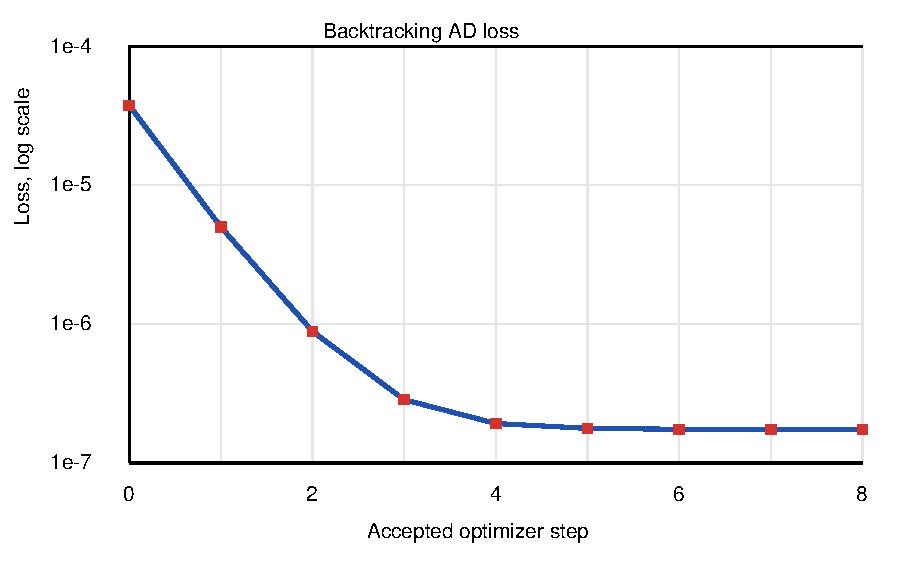
\includegraphics[width=3.2in]{backtracking_loss}
\caption{Backtracking AD optimizer loss trajectory for the clean off-grid
target. The nine recorded losses are
\(3.761{\times}10^{-5}\), \(5.013{\times}10^{-6}\),
\(8.864{\times}10^{-7}\), \(2.855{\times}10^{-7}\),
\(1.925{\times}10^{-7}\), \(1.775{\times}10^{-7}\),
\(1.749{\times}10^{-7}\), \(1.743{\times}10^{-7}\), and
\(1.740{\times}10^{-7}\).}
\label{fig:loss}
\end{figure}

The result also shows why inverse claims must report both field loss and
parameter error. Backtracking AD obtains the lowest field loss, but the dense
grid candidate is closer to the generating parameters on the clean case.

\subsection{Noise Sensitivity}
Grid recovery is stable through noise amplitude 0.020 across four deterministic
seeds. At amplitude 0.050, two of four seeds move to a neighboring candidate; at
0.100, three of four seeds move away from the clean candidate. Backtracking AD
remains competitive with grid-search noisy loss through 0.100 and keeps lower
clean-target loss in the noisy failure cases.

\begin{table}[!t]
\renewcommand{\arraystretch}{1.15}
\caption{Noise Sensitivity Summary Across Four Seeds}
\label{tab:noise}
\centering
\begin{tabular}{lccc}
\hline
Noise & Grid clean candidate & Grid shifted & AD-line stable\\
\hline
0.000 & 4/4 & 0/4 & 4/4\\
0.020 & 4/4 & 0/4 & 4/4\\
0.050 & 2/4 & 2/4 & 4/4\\
0.100 & 1/4 & 3/4 & 4/4\\
\hline
\end{tabular}
\end{table}

Here ``grid clean candidate'' means the dense grid returns the same
\((F,k)=(0.060500,0.062500)\) candidate recovered without noise. ``AD-line
stable'' means the backtracking AD optimizer remains in the same final parameter
region across all four deterministic seeds.

\subsection{Browser Inverse Performance}
The full AD-line inverse loop runs in-browser via a Web Worker without GPU,
Python, or server-side compute. Table~\ref{tab:browser_inverse} reports
headless Chrome 147 timings for three grid sizes with 8 optimizer iterations
and 100 simulation steps. At \(64\times64\), recovery completes in 68 ms after
WASM initialization, at 7.6 ms per iteration. The final clean-target loss of
\(1.740\times10^{-7}\) matches the native result, confirming numerical
consistency across the JS/WASM boundary. A \texttt{worker: true} flag in the
returned status JSON confirms off-thread execution.

\begin{table}[!t]
\renewcommand{\arraystretch}{1.15}
\caption{Browser Inverse Recovery Timing (HeadlessChrome 147, Web Worker,
8 Iterations, 100 Steps)}
\label{tab:browser_inverse}
\centering
\begin{tabular}{lcccc}
\hline
Grid & Eval. & Elapsed ms & ms/iter & Clean loss\\
\hline
\(32^2\) & 21 & 22.2 & 2.47 & \(6.884{\times}10^{-7}\)\\
\(64^2\) & 17 & 68.0 & 7.56 & \(1.740{\times}10^{-7}\)\\
\(96^2\) & 17 & 142.8 & 15.87 & \(1.737{\times}10^{-7}\)\\
\hline
\end{tabular}
\end{table}

\section{Discussion}
The experiments support three claims. First, Rust and WebAssembly can host a
validated interactive Gray--Scott solver without sacrificing deterministic
native testing. Second, forward-mode AD is a practical improvement over central
finite differences for a two-parameter inverse query. Third, optimizer mechanics
matter: a standard Armijo backtracking rule turns a weak fixed-step AD optimizer
into a competitive inverse method.

The current method is not a general differentiable PDE framework. Forward-mode
AD scales with the number of parameters, and the \(2.6\times\) overhead already
shows memory pressure from carrying tangent fields. Larger parameter spaces
would motivate adjoint or reverse-mode methods.

\section{Limitations}
The inverse task uses a fixed initial condition, two scalar parameters, and final
field MSE. The experiments do not yet establish robustness to unknown initial
conditions, observational masks, different time horizons, or real measurement
noise. SIMD and browser measurements are from a single machine, with browser
measurements running in headless Chrome; interactive and cross-browser
validation are left to future work. The browser inverse loop was not tested
under network latency or mobile constraints.

\section{Conclusion}
This paper presents a validated Rust/WebAssembly Gray--Scott implementation with
browser rendering benchmarks, WebAssembly SIMD acceleration, and differentiable
inverse recovery. Forward-mode AD gives a measured gradient-cost advantage over
finite differences, and Armijo backtracking AD recovers low-loss parameters with
far fewer evaluations than a dense grid search. The result is a compact,
reproducible platform for interactive differentiable reaction--diffusion
experiments.
A WASM \texttt{simd128} kernel achieves \(7\times\)--\(8.6\times\) speedup over
scalar WASM in Node.js, and the full differentiable inverse loop completes in
68 ms off the main browser thread via a Web Worker for a \(64\times64\) grid.

\section*{Acknowledgment}
The author thanks the open-source Rust and WebAssembly communities whose tooling
made this work possible.

\ifCLASSOPTIONcaptionsoff
  \newpage
\fi

\bibliographystyle{IEEEtran}
\bibliography{references}

\end{document}
